\documentclass{article}

% if you need to pass options to natbib, use, e.g.:
%     \PassOptionsToPackage{numbers, compress}{natbib}
% before loading neurips_2019

% ready for submission
%\usepackage{neurips_2019}

% to compile a preprint version, e.g., for submission to arXiv, add add the
% [preprint] option:
%     \usepackage[preprint]{neurips_2019}

% to compile a camera-ready version, add the [final] option, e.g.:
\usepackage[preprint, nonatbib]{neurips_2019}


\usepackage[utf8]{inputenc} % allow utf-8 input
\usepackage{hyperref}       % hyperlinks
\usepackage{url}            % simple URL typesetting
\usepackage{booktabs}       % professional-quality tables
\usepackage{amsfonts}       % blackboard math symbols
\usepackage{amsmath}
\usepackage{graphicx,wrapfig,lipsum}
\usepackage{amsfonts}
\usepackage{booktabs}
\usepackage{empheq}
\usepackage{amsthm}
\usepackage{caption}
\usepackage{subcaption}
\usepackage{mathrsfs}  
\usepackage{amssymb}
\usepackage{tikz}
\usetikzlibrary{calc,positioning}

%\usepackage{nicefrac}       % compact symbols for 1/2, etc.
%\usepackage{microtype}      % microtypography
%\usepackage[title]{appendix}

\hyphenpenalty=10000

\theoremstyle{plain}
\newtheorem{thm}{Theorem}[section]
\newtheorem{proposition}[thm]{Proposition}
\newtheorem{lemma}[thm]{Lemma}
\newtheorem{corollary}[thm]{Corollary}

\theoremstyle{definition}
\newtheorem{definition}[thm]{Definition}
\newtheorem{remark}[thm]{Remark}
\newtheorem{example}[thm]{Example}

\newcommand{\set}[2]{\left\{#1\,\left\vert\,#2\vphantom{#1}\right\}\right.}
\newcommand{\reals}{\mathbb{R}}
\newcommand{\naturals}{\mathbb{N}}
\newcommand{\bigO}{\mathcal{O}}
\newcommand{\norm}[1]{\mathord|\!\mathord|#1\mathord|\!\mathord|} % TODO: replace
\newcommand{\restr}[2]{{\left.\kern-\nulldelimiterspace #1 \right|_{#2}}}
\newcommand{\dee}{\,\mathrm{d}}
\newcommand{\logsig}{\mathrm{LogSig}}
\newcommand{\mfc}{\mathrm{MFC}}
\newcommand{\argmin}{\mathop\mathrm{argmin}\limits}
\newcommand{\boldheading}[1]{

\textbf{#1}\quad}

\title{Generalised Interpretable Shapelets for Irregular Time Series}

\author{
	\And
	Terry Lyons$^{1, 2}$
	\AND \\[-12pt]
	\null$^1$ Mathematical Institute, University of Oxford \\
	\null$^2$ The Alan Turing Institute, British Library \\
	\texttt{\{tlyons\}@\hspace{0.1pt}maths.ox.ac.uk}
}

% Notation:
% n index of N samples
% k index of K shapelets
% t index of S or T_n length
% s index of offset
% d index of D channels
% i index of I, the size of the wavelet basis

% TODO: need way more this-is-cool
% TODO: make sure this handles irregularly sampled time series properly
\begin{document}
	\maketitle
	\begin{abstract}
		The shapelet transform is a form of feature extraction for time series, in which a time series is described by its similarity to each of a collection of `shapelets'. However existing work has suffered from several limitations, such as fragility to noise, loss of interpretability, and a dependence on fully observed and regularly sampled data. In this work, we demonstrate how the shapelet transform may be improved and generalised in multiple ways: by using learnt pseudometrics as a measure of similarity between time series; by demonstrating that a regularisation penalty ensures interpretability; by allowing the length of each shapelet to be learnt differentiably (in contrast to its previously discrete formulation). Furthermore our \emph{generalised shapelet transform} is applicable to the general case of irregularly sampled partially observed multivariate time series. We validate our method by demonstrating its empirical performance on several datasets.
	\end{abstract}
	\section{Introduction}
	Shaplets are a form of feature extraction for time series. Given some fixed hyperparameter $K$, describing how many shapelets we are willing to consider, then each time series is represented by a vector of length $K$ describing how similar it is to each of the $k$ selected shapelets.
	
	We begin by stating the classical definition of shapelets.
	\subsection{Classical shapelets}
	Given $N$ regularly sampled multivariate time series, with $D$ observed channels, where the $i$-th time series is of length $T_n$, then the $n$-th time series is a matrix 
	\begin{equation}\label{eq:f-n}
	f^n = (f^n_{t})_{t \in \{0, \ldots, T_n - 1\}} = (f^n_{t, d})_{t \in \{0, \ldots, T_n - 1\}, d \in \{1, \ldots, d\}},
	\end{equation}
	with each $f^n_{t, d} \in \reals$. We assume without loss of generality that $0, \ldots, T_n - 1$ are the times at which each sample is observed, so that the parameterisation $t$ corresponds to the time of an observation.
	
	Fix some hyperparameter $K \in \naturals$, which will describe the number of shapelets. Fix some $S \in \{0, \ldots, \min_{i \in \{1, \ldots, N\}}T_n - 1\}$, which will describe the length of each shapelet. We define the $k$-th shapelet as a matrix
	\begin{equation*}
	w^{k} = (w^{k}_t)_{t \in \{0, \ldots, S - 1\}} = (w^{k}_{t, d})_{t \in \{0, \ldots, S - 1\}, d \in \{1, \ldots, d\}},
	\end{equation*}
	with each $w^{k}_{t, d} \in \reals$.
	
	Then the discrepancy between $f^n$ and $w^{k}$ is defined by:
	\begin{equation}\label{eq:classical-shapelets}
	\sigma_S(f^n, w^{k}) = \min_{s \in \{0, \ldots, T_n - S\}} \sum_{t = 0}^{S - 1} \norm{f^n_{s + t} - w^{k}_t}_2^2,
	\end{equation}
	where $\norm{\,\cdot\,}_2$ describes the $L^2$ norm on $\reals^D$. A small discrepancy implies that $f^n$ and $w^{k}$ are similar to one another. This corresponds to sweeping $w^{k}$ over $f^n$, and finding the offset $s$ at which $w^{k}$ best matches $f^n$. The collection of $(\sigma_S(f^n, w^{1}), \ldots, \sigma_S(f^n, w^{K})) \in \reals^K$ is now a feature describing $f^n$. This may now be passed to some model to perform classification or regression.
	
	In \cite{TODO}, a procedure is described for selecting shapelets as particular small intervals from particular training samples. However doing so is very expensive, requiring $\bigO(N^2 \cdot \max_n T_n^4)$ work. As such, \cite{TODO} instead show that the discrepancy $\sigma_S$ of equation \eqref{eq:classical-shapelets} is differentiable with respect to $w^{k, \rho, S}$, and so the shapelets may be selected differentiably\footnote{Although they include a `softmin' procedure which we believe to be unnecessary, as the minimum function is already almost everywhere differentiable.}, as part of an end-to-end optimisation of the final loss function of the model that uses the shapelets as features.
	
	The shapelet method is attractive for three reasons. First, it is invariant to the value of $T_n$, and as such provides a way to normalise variable-length time series. Second, it is interpretable, as use of a particular feature corresponds to the importance of the similarity to the shapelet $w^{k}$, which may for example describe some shape that is characteristic of a particular class; furthermore the value of $s$ gives where the similarity occurs. Third, it typically demonstrates good performance \cite{TODO}.
	
	\subsection{Limitations}
	However, classical shapelet methods also suffer from a number of limitations.
	\begin{enumerate}
	\item The technique only applies to regularly spaced time series, due to the minimisation over $s$. 
	\item The choice of $S$ is a hyperparameter; it is discrete, and choosing it is thus a relatively expensive optimisation procedure.
	\item The technique is not robust to irrelevant channels (which will typically exist in many real world datasets, for example medical time series): equation \eqref{eq:classical-shapelets} attempts to fit a $w^{k}_{t, d}$ even for uninformative channels $d$.
	\item Selecting $w^{k}$ is either expensive, following the procedure of \cite{TODO}, or loses interpretability, following the procedure of \cite{TODO}.  % TODO: there's also the adversarial interpretability paper that seems a bit naff
	\item The formulation of equation \eqref{eq:classical-shapelets} has essentially made several ad-hoc choices, for example in the choice of $L^2$ norm on $\reals^D$. Indeed, there are many natural notions of discrepancy between time series \cite{TODO, TODO, TODO, TODO} that do not fit this framework.
	\end{enumerate}
	
	\subsection{Contributions}
	We demonstrate how classical shapelets may be generalised in multiple ways, so as to address the collection of limitations just described.
	
	We demonstrate how the discrepancy between a shapelet and a time series may be taken to be a learnt pseudometric; this makes our proposed method robust to noise in unrelated channels, and additionally introduces a great deal of flexibility into the method. Furthermore, we demonstrate how simple regularisation is enough to achieve shapelets that resemble characteristic features of the data, in order to achieve the desired interpretability.
	
	Additionally, by treating the objects in continuous time rather than discrete time, we demonstrate how the length of each shapelet may be learnt, individually for each shapelet, in a differentiable manner. This continuous-time formulation also allows our \emph{generalised shapelet transform} to extend to the general case of irregularly sampled partially observed multivariate time series.
	
	Our code is available at TODO.
	
	\section{Method}
	We move on to describing our method, which we present in a general form. In the next section we will discuss the specific choices made in our experiments.
	
	\subsection{Continuous-time objects}
	We interpret a time series as a discretised sample from an underlying process, observed only through the time series. Similarly, the shapelet previously constructed may be thought of as a discretisation of some underlying function. The first important step in our procedure is to construct continuous-time approximations to these underlying objects.
	
	\boldheading{Continuous-time path interpolants}
	Formally speaking, we assume that for $n \in \{1, \ldots, N\}$ indexing different time series, we observe a collection of time series
	\begin{equation*}
	f^n = (f^n_{t_\tau})_{\tau \in \{1, \ldots, T_n\}},
	\end{equation*}
	where $t_\tau \in \reals$ is the observation time of $f^n_{t_\tau} \in (\reals \cup \{*\})^D$, where $*$ denotes the possibility of a missing observation. This description allows irregularly sampled partially observed time series to be treated on the same footing as regularly sampled and completely observed time series.
	
	Next, interpolate to get a function $\iota(f^n) \colon [0, T_n - 1] \to \reals^D$ such that $\iota(f^n)(t_\tau) = f^n_{t_\tau}$ for all $\tau \in \{0, \ldots, T_n - 1\}$ such that $f^n_{t_\tau}$ is observed. There are many possible choices for interpolations, for example splines \cite{TODO}, kernel methods \cite{interpolation-prediction}, or Gaussian processes \cite{gp-adapter1, gp-adapter2}. In our experiments, we use piecewise linear interpolation.
	
	\boldheading{Continuous-time shapelets}
	The shapelets themselves we are free to control, and so for $k \in \{1, \ldots, K\}$ indexing different shapelets, we take each $w^{k, \rho} \colon [0, 1] \to \reals^D$ to be some learnt function depending on learnt parameters $\rho$. For example, this could be an interpolated sequence of learnt points, an expansion in some basis functions, or a neural network. In our experiments we use linear interpolation of a sequence of a learnt points.
	
	Then for some learnt length $S_k > 0$, define $w^{k, \rho, S_k} \colon [0, S_k] \to \reals^D$ by
	\begin{equation*}
	w^{k, \rho, S_k}(t) = w^{k, \rho}\left(\frac{t}{S_k}\right).
	\end{equation*}
	Taking the length $S_k$ to be continuous is a necessary prerequisite to training it differentiably. We will discuss the training procedure in a moment.
	
	\subsection{Generalised discrepancy}
	The core of the shapelet method is that the similarity or discrepancy between $f^n$ and $w^{k, \rho, S_k}$ is important. In general, we approach this by defining a \emph{discrepancy function} between the two, which will typically be learnt, and which we require only to be a pseudometric, rather than a metric. By relaxing to allow pseudometricity, then the procedure becomes robust to noise in unrelated channels, as the learning procedure may learn to ignore extraneous dimensions.
	
	We denote this discrepancy function by $\pi^A_{S_k}$; it depends upon the length $S_k$ and a learnt parameter $A$, consumes two paths in $\reals^D$, and returns a real number describing some notion of closeness between them. We are being deliberately vague about the domain of $\pi^A_{S_k}$, as it is a function space whose regularity will depend on $\iota$.	
	
	Given some fixed $\pi^A_{S_k}$, then we define the discrepancy between $f^n$ and $w^{k, \rho, S_k}$ to be given by
	\begin{equation}\label{eq:new-sigma}
	\sigma^A_{S_k}(f^n, w^{k, \rho, S_k}) = \min_{s \in [0, T_n - S_k]} \pi^A_{S_k}(\restr{\iota(f^n)}{[s, s + S_k]}(s + \cdot), w^{k, \rho, S_k}).
	\end{equation}
	
	The collection of discrepancies $(\sigma^A_{S_k}(f^n, w^{1, \rho, S_k}), \ldots, \sigma^A_{S_k}(f^n, w^{K, \rho, S_k}))$ is now a feature describing $f^n$, and is invariant to the length $T_n$. Use of the particular feature $\sigma^A_{S_k}(f^n, w^{k, \rho, S_k})$ corresponds to the importance of the similarity between $f^n$ and $w^{k, \rho, S_k}$. In this way, the choice of $\pi^A_{S_k}$ gives a great deal of flexibility: not only may it be selected for reasons of classification performance, but it may also be selected to aid interpretability, as we are about to see.
	
	\boldheading{Existing shapelets fit into this framework}
	A simple example, in analogy to the classical shapelet method of equation \eqref{eq:classical-shapelets}, is to take
	\begin{equation*}
	\pi^A_{S_k}(f, w) = (\int_{0}^{S_k} \norm{f(t) - w(t)}_2^2 \dee t)^{\frac{1}{2}},
	\end{equation*}
	which in fact has no $A$ dependence. If $\iota$ is taken to be a piecewise constant `interpolation' then this will exactly correspond to (the square root of) the classical shapelet approach.
	
	\boldheading{Learnt $L^2$ discrepancies}
	The previous example may be generalised by taking our learnt parameter $A \in \reals^{D \times D}$, and then letting
	\begin{equation}\label{eq:learnt-discrepancy}
	\pi^A_{S_k}(f, w) = (\int_{0}^{S_k} \norm{A(f(t) - w(t))}_2^2 \dee t)^{\frac{1}{2}}.
	\end{equation}
	That is, allowing some learnt linear transformation before measuring the discrepancy. As we have allowed pseudometricity, then uninformative dimensions may be shrunk to zero. In our experiments we consider two possible formats for $A$: a general element of $\reals^{D \times D}$, or restricted to be diagonal. Being a general element allows for the possibility of dimensions to interact with one another, but whether this is beneficial is likely to be problem-dependent.
	
	\boldheading{More complicated discrepancies}
	Moving on, we consider other more general choices of discrepancy, which may be motivated by the problem at hand. In particular we will discuss discrepancies based on the logsignature transform \cite{TODO}, and mel-frequency cepstrums (MFC) \cite{TODO}.
	
	Our exposition on these two discrepancies will be deliberately brief, as the finer details on exactly when and how to use the logsignature and MFC transforms is not important to us here. The point is that our framework has the flexibility to consider general discrepancies motivated by other discplines, or which are known to extract information which is particular useful to the domain in question. An understanding of either logsignatures or mel-frequency cepstral coefficients will not be necessary to follow this paper.
	
	\boldheading{Logsignature discrepancies}
	The logsignature transform is a transform on paths, known to characterise its input whilst extracting statistics which describe how the path controls differential equations \cite{levy-lyons, deep-signatures, signatory, logsig-rnn}. Let $\mu$ denote the M{\"o}bius function, and let
	\begin{equation*}
	\beta_{D, R} = \sum_{r = 1}^R \frac{1}{r} \sum_{\rho \vert r} \mu\left(\frac{r}{\rho}\right) D^\rho
	\end{equation*}
	which is Witt's formula \cite{witt}. Let
	\begin{equation*}
	\logsig^R \colon \set{f \colon [0, T] \to \reals^D}{T \in \reals, f\text{ is of bounded variation}} \to \reals^{\beta_{D, R}}
	\end{equation*}
	be the depth-$R$ logsignature transform. Let $A \in \reals^{\beta_{D, R} \times \beta_{D, R}}$ be full or diagonal as before, and let $\norm{\,\cdot\,}_p$ be the $L^p$ norm on $\reals^{\beta_{D, R}}$. Then we define the \emph{$p$-logsignature discrepancy} between two functions to be
	\begin{equation}\label{eq:logsignature-discrepancy}
	\pi^A_{S_k}(f, w) = \norm{A(\,\logsig^R(f) - \,\logsig^R(w))}_p.
	\end{equation}
	
	\boldheading{MFC discrepancies}
	The computation of a MFC is a function-to-function map derived from the short-time Fourier transform, using additional processing to focus on information that is particularly relevant to human hearing. Letting $\mfc$ represent the computation of an MFC, then we compose this with the $L^2$ based discrepancy of equation \eqref{eq:learnt-discrepancy} to produce
	\begin{equation}\label{eq:mfc-discrepancy}
	\pi^A_{S_k}(f, w) = (\int_{0}^{S_k} \norm{A(\mfc(f)(t) - \mfc(w)(t))}_2^2 \dee t)^{\frac{1}{2}}.
	\end{equation}
	
	\boldheading{The generalised shapelet transform}
	Whatever the choice of $\pi^A_S$, and in analogy to classical shapelet methods, we call the map
	\begin{equation*}
	f \mapsto (\sigma^A_{S_1}(f, w^{1, \rho, S_1}), \ldots, \sigma^A_{S_K}(f, w^{K, \rho, S_K}))
	\end{equation*}
	the \emph{generalised shapelet transform}.
	
	\subsection{Interpretable regularisation}
	Selecting shapelets by searching as in \cite{TODO} is incredibly expensive. Selecting them as part of a differentiable optimisation procedure is much more attractive for its speed, and is faciliated by deep learning tools that typically optimise in the same way. However, it has been noted in \cite{TODO} that this method sacrifices much of the interpretability, as the shapelets that are then selected need not look like any small extracts from the training data. 
In \cite{TODO} they propose to solve this issue via adversarial regularisation.

	We instead propose a much simpler method; train differentiably as before, and add on
	\begin{equation}
		\label{eq:interpretable_reg}
		\sum_{k = 1}^K \min_{n \in \{1, \ldots, N\}} \sigma^A_S(f^n, w^{k, \rho, s})
	\end{equation}
	as a regularisation term, so that minimising the discrepancy between $f^n$ and $w^{k, \rho, S}$ is also important. Note the choice of minimisation over $n$, rather than a sum over $n$. A sum over $n$ would ask that every shapelet should look like every training sample. Taking a minimum instead asks only that every shapelet should be similar to a single training sample.
	
	\subsection{Minimisation objective and training procedure}
	Overall, suppose we have some parametric (typically linear) model $F^\theta$, some loss function $\mathcal{L}$, and some observed time series $f^1, \ldots, f^N$ with targets $y_1, \ldots, y_N$.	
	
	Then letting $\gamma > 0$ control the amount of regularisation, we propose to minimise
	\newcommand{\objective}{&\frac{1}{N}\sum_{n = 1}^N \mathcal{L}(y_n, F^\theta(\sigma^A_{S_1}(f^n, w^{1, \rho, S_1}), \ldots, \sigma^A_{S_K}(f^n, w^{K, \rho, S_K}))) + \gamma \sum_{k = 1}^K \min_{n \in \{1, \ldots, N\}} \sigma^A_{S_k}(f^n, w^{k, \rho, S_k})}
	\begin{align}
	\objective \label{eq:objective}
	\end{align}
	over model parameters $\theta$, discrepancy parameters $A$, shapelet parameters $\rho$, and shapelet lengths $S_k$, via standard stochastic gradient descent based techniques.
	
	\boldheading{Differentiability}
	Some thought is necessary to verify that our constructions are in fact differentiable, and in particular differentiable with respect to $S_k$. Examining the definition of $\sigma^A_{S_k}$ in equation \eqref{eq:new-sigma}, there are also two operations that may seem to pose a problem, namely the restriction operator $\iota(f^n) \mapsto \restr{\iota(f^n)}{[s, s + S_k]}$, and the minimum over a range $\min_{s \in [0, T_n - S_k]}$; neither of these are a standard part of an autodifferentiation framework such as PyTorch \cite{pytorch}.
	
	Practically speaking, however, it is straightforward to resolve all of these issues. The continuous-time paths $\iota(f^n)$ and continuous-time shapelets $w^{k, \rho, S_k}$ must both be represented by some parameterisation of function space, and it is thus sufficient to restrict to considering differentiability with respect to this parameterisation. In our experiments we represent both $\iota(f^n)$ and $w^{k, \rho, S_k}$ as a continuous piecewise linear function stored as a collection of knots.
	
	In this context, the restriction operator is clearly differentiable, as a map from the unrestricted function, represented by one collection of knots, to the restricted function, represented by another collection of knots. Each knot is either kept (the identity function), thrown away (the zero function), or interpolated between to place a new knot at the boundary (a ratio of existing knots), and so collectively the map is differentiable.
	
	For the minimum over a range, this may reasonably be approximated by a minimum over some collection of points $s \in \{0, \varepsilon, 2 \varepsilon, \ldots, T_n - S_k - \varepsilon, T_n - S_k\}$, for some $\varepsilon > 0$ small and dividing $T_n - S_k$. This is now a standard piece of an autodifferentiation package. The error of this approximation may be controlled by the modulus of continuity of $s \mapsto \pi^A_{S_k}(\restr{\iota(f^n)}{[s, s + S_k]}(s + \cdot), w^{k, \rho, S_k})$, but in practice we found this to be unnecessary, and simply took $\varepsilon$ equal to the smallest gap between observations.
	
	\boldheading{Choice of $F^\theta$}
	Interpretability of the model will depend on an interpretable choice of $F^\theta$. In our experiments we took a natural logarithm of every feature, and then used a linear model. The logarithm is because the discrepancies $\sigma^A_{S_k}(f^n, w^{k, \rho, S_k}) \in [0, \infty)$, so the logarithm maps this to $\reals$. (As a technical point, a small number such as $10^{-5}$ may need to first be added to prevent $\log \colon 0 \mapsto -\infty$.)
	
	This is now easily interpretable: a very negative coefficient of $\log \sigma^A_{S_k}(f^n, w^{k, \rho, S_k})$ corresponds to the importance of $\sigma^A_{S_k}(f^n, w^{k, \rho, S_k})$ being close to zero, and thus the importance of $f^n$ and $w^{k, \rho, S_k}$ being similar to each other.
	
	
	\section{Experiments}
Our generalised shapelet transform, contrasted with the classical shapelet transform, has two extra degrees of freedom: the choice of interpolation scheme $\iota$, and the choice of discrepancy function $\pi^A_S$. In our experiments, we consider $\pi^A_S$ given by either of equations \eqref{eq:learnt-discrepancy} or \eqref{eq:logsignature-discrepancy} and in both cases take the discrepancy parameters $A$ to be diagonal, as this was empirically found empirically to perform best, and the truncation depth of the log-signature is always taken to be $3$. Meanwhile, we take $\iota$ to be piecewise linear interpolation, because efficient algorithms for computing the logsignature transform only exist for piecewise linear paths \cite{signatory}.

For old shapelets, the key hyperparameters to consider are the number of shapelets and the length the these shapelets correspond to. A full description of the hyperparameter selection process is given in Appendix \ref{}. In short we perform a small hyperparameter search for each dataset to optmise the number and length of the shapelets for the old method and use these same parameters in the generalised approach. The length hyperparameter has less meaning in the generalised approach as it is changed during the learning process, but is used in the shapelet initialisation scheme such that the initialised shapelts are the same in all cases.

\subsection{The UEA (Multivariate) Time-Series Archive}
We begin by comparing the classification performance of the old method of shapelets to our new `generalised' approach for which we consider three learnt metrics: a standard L2-metric, an learnt metric and a logsig-3-diagonal. We evaluate the methods on a subset of the UEA time-series archive \cite{bagnall2018uea}. This contains a wide range of multivariate time-series classification problems from various fields with significant differences in time-series length, number of classes, and amount of training data. The full collection contains 30 datasets, however due to algorithm run-time constraints we have considered a subset of these ensuring they still contain significant variation. The statistics of these datasets are given in Table \ref{} of the Appendix.

The results are given in Table \ref{tab:uea_comparison_results}. We see significantly improved classification performance ($> 1$ standard deviation) on $6$ of the $9$ datasets tested with $1$ draw and $2$ losses. We note that the loss on `PenDigits' was extemely close, and the other loss was on `BasicMotions' which has a very small total number samples ($80$) making overfit more likely on the generalised methods (without proper hyperparameter tuning) due to the additional parameters in the model. In contrast, there are many cases where the new method won with significantly higher accuracies than the old method. We also note that the method is sensitive to choice of hyperparameters, and all hyperparameters were chosen for the old method, if hyperparameters were chosen separately for each discrepancy, this would likely improve the results for the learnt discrepancies further.
\begin{table}[ht]
    \centering
    \caption{Classification performance on the UEA datasets from the old shapelet method and the generalised method with a diagonal L2 and diagonal logsig metric with depth 3. The values indicate the classification accuracy on the test set plus or minus one standard deviation. The wins are computed as the number of times each algorithm was within 1 standard deviation from the top score for each dataset.}
    \label{tab:uea_comparison_results}
    \begin{tabular}{lccc}
\toprule
{} & \multicolumn{3}{c}{\textbf{Discrepancy}} \\
\textbf{Dataset} &          L2-diagonal &   logsig-3diagonal &                old \\
\midrule
BasicMotions    &    0.908 $\pm$ 0.014 &  0.808 $\pm$ 0.038 &  0.967 $\pm$ 0.058 \\
ERing           &    0.826 $\pm$ 0.063 &  0.433 $\pm$ 0.029 &  0.672 $\pm$ 0.118 \\
Epilepsy        &    0.884 $\pm$ 0.030 &  0.886 $\pm$ 0.008 &  0.729 $\pm$ 0.054 \\
Handwriting     &    0.103 $\pm$ 0.026 &  0.118 $\pm$ 0.012 &  0.065 $\pm$ 0.037 \\
JapaneseVowels  &    0.972 $\pm$ 0.011 &  0.539 $\pm$ 0.030 &  0.915 $\pm$ 0.041 \\
LSST            &    0.361 $\pm$ 0.002 &  0.357 $\pm$ 0.004 &  0.335 $\pm$ 0.005 \\
Libras          &    0.670 $\pm$ 0.094 &  0.678 $\pm$ 0.055 &  0.622 $\pm$ 0.024 \\
PenDigits       &    0.973 $\pm$ 0.001 &  0.967 $\pm$ 0.007 &  0.975 $\pm$ 0.006 \\
RacketSports    &    0.796 $\pm$ 0.007 &  0.612 $\pm$ 0.092 &  0.796 $\pm$ 0.024 \\ 
\midrule
Wins &            5 &                 3 &    3 \\
\bottomrule
\end{tabular}

\end{table}


\subsubsection{Algorithm Interpretability}
Here we explore the effect of the inclusion of the regularisation term from Equation \cite{eq:interpretable_reg} on shapelet interpretability. Recall that the term was chosen to ensure the resulting shapelets are `close', in the sense of the chosen discrepancy, to some subsample of the training data. To examine this we consider the PenDigits dataset where participants were asked to write down a number from 0-9 and the goal is to classify the intended digit. In Figure \ref{fig:pendigits} we plot, for each digit (0 to 9 in order from left to right), the learnt shapelet that corresponds to the largest coefficient from the logistic-regression for that class. For the old method \ref{fig:old_shapelets}, it is in general not clear what aspect of the digit the shapelet is representing. In some cases the closest digit to the shapelet is not even of the class for which it is thought to best discriminate. Furthermore, the 0 and 1 classes along with the 5 and 8 classes share their `top' shapelet. In contrast, it is abundantly clear what aspect of the digit is being captured by the top shapelets produced from our generalised method \ref{fig:new_shapelets}. Some particular points of interest include shape of the 5 and 6 shapelet being very similar, but the distinction being found in the shapelets chirality (along with its thickness) as the bottom half of a 5 is written clockwise and the 6 anticlockwise. The shapelet for the 7 digit is interesting in its simplicity with it not being immediately clear what makes it so discriminative. By considering those digits with strokes in the top left hand region, we can see that the 8 and 9 have different chiralities to the 7, and the strokes for 1, 2 and 3 are generally written curving upwards to being with wheras 7 is usually flat. A similar such case can be made to explain why the shapelet for the 2 is found to be highly discriminative.

We chose PenDigits here because it is easy to understand visually what the shapelet represents. In general this is not the case, but provided we can make sense of isolated subintervals of the time-series, then the generated results will be interpretable in this context.
\begin{figure}[ht]
    \begin{subfigure}[b]{\linewidth}
        \centering
        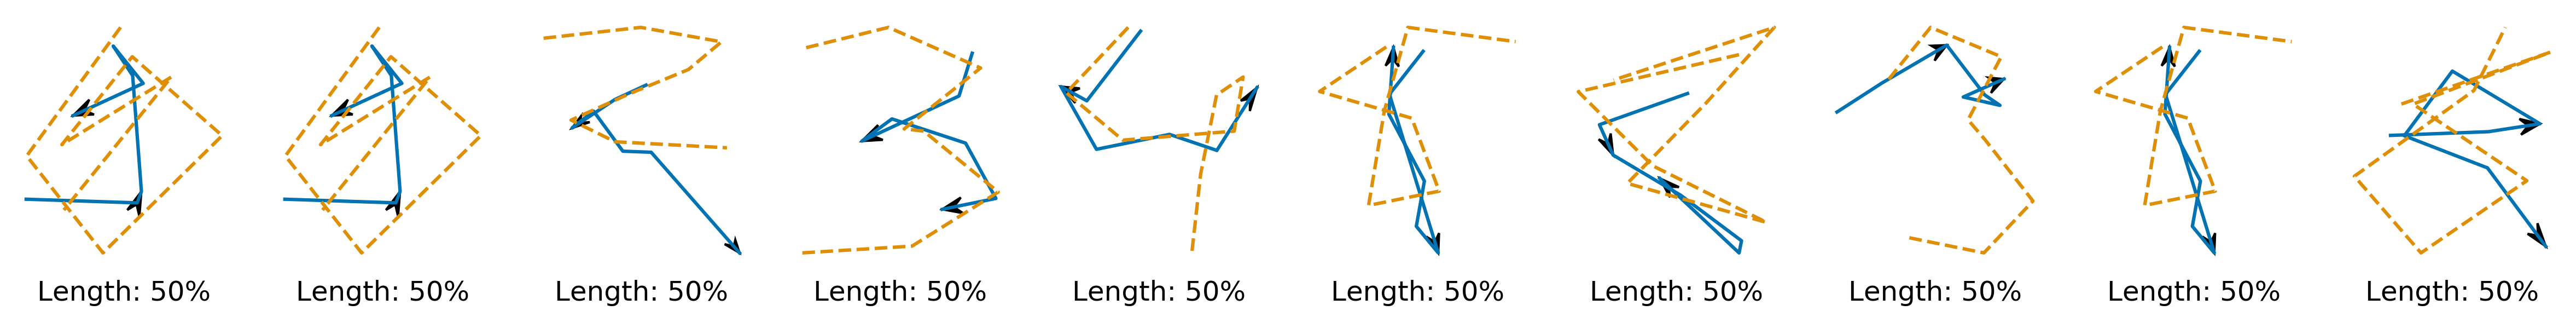
\includegraphics[width=\linewidth]{images/pendigits/old_shapelets_noborder.png}
        \caption{Old shapelets.}
        \label{fig:old_shapelets}
    \end{subfigure}
    \begin{subfigure}[b]{\linewidth}
        \centering
        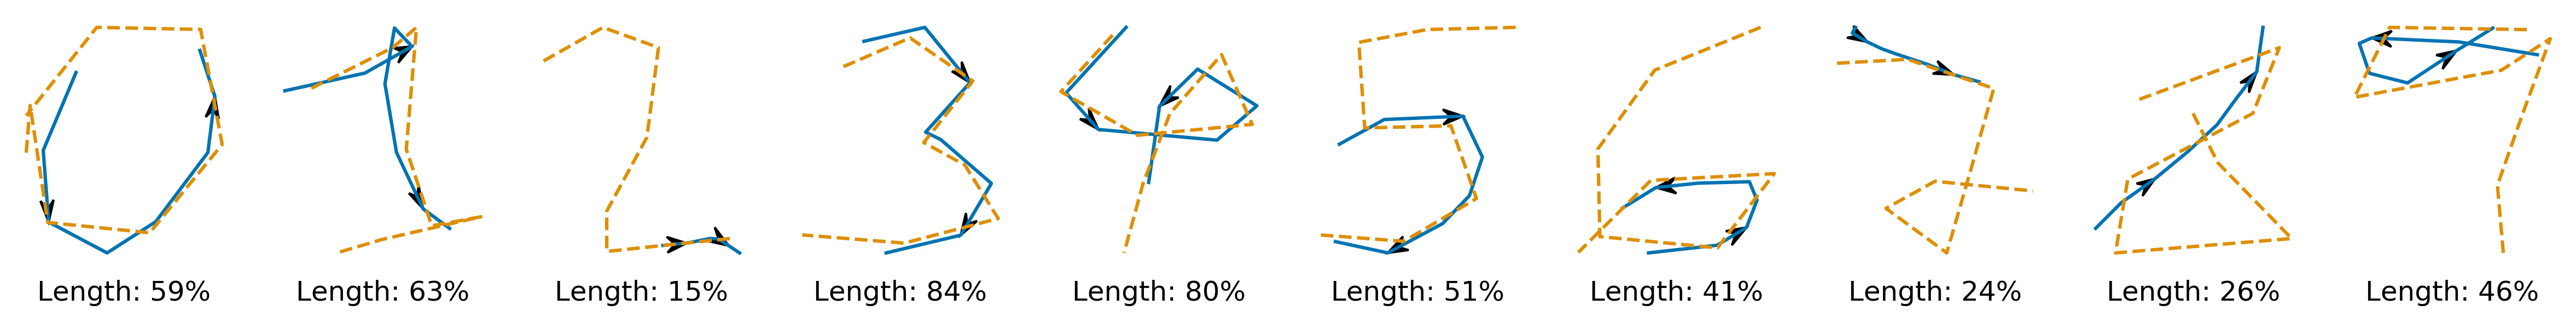
\includegraphics[width=\linewidth]{images/pendigits/new_shapelets_noborder.png}
        \caption{New shapelets.}
        \label{fig:new_shapelets}
    \end{subfigure}
    \caption{The learnt shapelet that corresponds to the largest coefficient in the logistic regression layer for the digits 0 to 9 in order from left to right (blue) and the `closest' path (the path with smallest discrepancy) from the training data (orange dashed).}
    \label{fig:pendigits}
\end{figure}


\subsubsection{Missing Data and Length Ablation}
We now demonstrate both the ability of the proposed framework to handle partially observed data, as well as show the effectiveness of having learnable shapelet lengths.
\begin{table}[ht]
    \caption{}
    \label{tab:uea_noise}
    \centering
    \begin{tabular}{lcccc}
\toprule
{} & \multicolumn{4}{c}{\textbf{Discrepancy}} \\
\textbf{Dataset} &       logsig-3-False &           L2-False &      logsig-3-True &            L2-True \\
\midrule
BasicMotions10    &    0.783 $\pm$ 0.038 &  0.933 $\pm$ 0.038 &  0.767 $\pm$ 0.101 &  0.883 $\pm$ 0.118 \\
BasicMotions30    &    0.825 $\pm$ 0.050 &  0.958 $\pm$ 0.029 &  0.758 $\pm$ 0.063 &  0.942 $\pm$ 0.029 \\
BasicMotions50    &    0.733 $\pm$ 0.115 &  0.942 $\pm$ 0.038 &  0.733 $\pm$ 0.063 &  0.925 $\pm$ 0.066 \\
JapaneseVowels10  &    0.677 $\pm$ 0.082 &  0.955 $\pm$ 0.037 &  0.634 $\pm$ 0.017 &  0.950 $\pm$ 0.034 \\
JapaneseVowels30  &    0.639 $\pm$ 0.025 &  0.968 $\pm$ 0.001 &  0.628 $\pm$ 0.063 &  0.969 $\pm$ 0.002 \\
JapaneseVowels50  &    0.611 $\pm$ 0.061 &  0.968 $\pm$ 0.003 &  0.620 $\pm$ 0.006 &  0.966 $\pm$ 0.003 \\
LSST10            &    0.365 $\pm$ 0.005 &  0.363 $\pm$ 0.001 &  0.359 $\pm$ 0.009 &  0.358 $\pm$ 0.007 \\
LSST30            &    0.360 $\pm$ 0.007 &  0.360 $\pm$ 0.001 &  0.360 $\pm$ 0.007 &  0.407 $\pm$ 0.010 \\
LSST50            &    0.354 $\pm$ 0.007 &  0.362 $\pm$ 0.008 &  0.358 $\pm$ 0.004 &  0.381 $\pm$ 0.034 \\ 
\midrule
Wins &               1 &         5 &              0 &        4 \\
\bottomrule
\end{tabular}

\end{table}


\subsection{Speech Commands}
Finally we examine the performance on the speech commands dataset \ref{warden2018speech} which includes a selection of one-second audio files with each representing a single spoken word. The aim is to build a model to detect the word that has been spoken. We chose this dataset as it is significantly larger than any in the UEA archive so as to demonstrate that the method is not restricted to these (relatively) small datasets. We do reiterate that the computational cost of shapelet methods is high in comparison to other more traditional deep-learning approaches and so can make datasets such as this prohibitive, in particular, it is why we have left the logsig-3 discrepancy out of our analysis in this instance as it takes significantly longer to train compared with the L2 methods.
\begin{table}[ht]
    \caption{Classification accuracy for old shapelets and new shapelets on the Speech Commands dataset.}
    \label{tab:speech_commands}
    \centering
    \begin{tabular}{cc}
\toprule
\multicolumn{2}{c}{Discrepancy} \\
Old &  L2 \\
\midrule
- & - \\
- & - \\
\bottomrule
\end{tabular}

\end{table}

\subsubsection{Interpretability of Speech Commands}
Pray for me.




	\section{Conclusion}


\end{document}
